%-------------------------
% Resume in Latex
% Author : Audric Serador
% Inspired by: https://github.com/sb2nov/resume
% License : MIT
%------------------------

\documentclass[letterpaper,11pt]{article}
% \usepackage[top=1in,bottom=1in,left=1in,right=0.5in]{geometry}
\usepackage{fontawesome5}
\usepackage{latexsym}
\usepackage[empty]{fullpage}
\usepackage{titlesec}
\usepackage{marvosym}
\usepackage[usenames,dvipsnames]{color}
\usepackage{verbatim}
\usepackage{enumitem}
\usepackage[hidelinks]{hyperref}
\usepackage{fancyhdr}
\usepackage[english]{babel}
\usepackage{tabularx}
\usepackage{multicol}
\usepackage{ragged2e}
\usepackage{tikz}
\usepackage{newtxtext,newtxmath} % Times New Roman (recommended)
\usepackage{xstring}
\input{glyphtounicode}


% Custom font
% \usepackage[default]{lato}

\pagestyle{fancy}
\fancyhf{} % clear all header and footer fields
\fancyfoot{}
\renewcommand{\headrulewidth}{0pt}
\renewcommand{\footrulewidth}{0pt}
\definecolor{bblue}{RGB}{70, 70, 205}
% \definecolor{bblue}{RGB}{0, 0, 0}

% Adjust margins
\addtolength{\oddsidemargin}{-0.5in}
\addtolength{\evensidemargin}{-0.5in}
\addtolength{\textwidth}{1in}
\addtolength{\topmargin}{-0.5in}
\addtolength{\textheight}{1in}

\urlstyle{same}

\raggedbottom
\raggedright
\setlength{\tabcolsep}{0in}
% Sections formatting
\titleformat{\section}{
  % \vspace{-4pt}\bfseries\scshape\centering\large\color{bblue}}
  \bfseries\scshape\raggedright\large\color{bblue}}
  {}
  {0em}
  {}
  [\titlerule]

% Ensure that generate pdf is machine readable/ATS parsable
\pdfgentounicode=1

%-------------------------%
% Custom commands
\begin{document}
%-------------------------%
% Custom commands
\newcommand{\resumeItem}[1]{
    \item\small{
        \parbox[t]{\dimexpr\textwidth-1.5in}{#1} % Use a parbox
    }
}

\newcommand{\resumeItemLong}[1]{
    \item\small{
        \parbox[t]{\dimexpr\textwidth-1in}{#1} % Use a parbox
    }
}

\newcommand{\resumeSubheading}[4]{
  \item
    \begin{tabular*}{0.97\textwidth}[t]{l@{\extracolsep{\fill}}r}
      \textbf{#1} & \footnotesize #2 \\ 
      \textit{\small #3}, \textit{\small #4}
    \end{tabular*}
}

\newcommand{\resumeSubheadingTwo}[2]{
  \item
    \begin{tabular*}{0.97\textwidth}[t]{l@{\extracolsep{\fill}}r}
      \textbf{#1} & \footnotesize #2 \\ 
    \end{tabular*}
}

\newcommand{\resumeSubSubheading}[2]{
    \item
    \begin{tabular*}{0.97\textwidth}{l@{\extracolsep{\fill}}r}
      \textit{\small#1} & \textit{\small #2} \\
    \end{tabular*}
}

\newcommand{\resumeProjectHeading}[2]{
    \item
    \begin{tabular*}{0.97\textwidth}{l@{\extracolsep{\fill}}r}
      #1 & {\footnotesize #2} \\
    \end{tabular*}
}

\newcommand{\resumeSubItem}[1]{\resumeItem{#1}}

\renewcommand\labelitemii{$\vcenter{\hbox{\small$\bullet$}}$}

\newcommand{\resumeSubHeadingListStart}{\begin{itemize}[leftmargin=0.15in, label={}, itemsep=2pt, parsep=0pt]}
\newcommand{\resumeSubHeadingListEnd}{\end{itemize}}
\newcommand{\resumeItemListStart}{\begin{itemize}[itemsep=2pt, parsep=0pt]}
\newcommand{\resumeItemListEnd}{\end{itemize}}

\definecolor{Black}{RGB}{0, 0, 0}
\definecolor{Blue}{RGB}{50, 50, 255}
\newcommand{\seticon}[1]{\textcolor{Blue}{\csname #1\endcsname}}

%-------------------------------------------%
%%%%%%  RESUME STARTS HERE  %%%%%

%----------HEADING----------%
    % \textbf{\huge \scshape Noam Smilovich} \\ \vspace{6pt}
    % %Machine Learning Engineer $\|$ Software Engineer $\|$ System Integration \\ \vspace{2pt}
    % \seticon{faPhone} \ \small 408-502-0772 \quad \\
    % \href{mailto:noam.smilovich@sjsu.edu}{\seticon{faEnvelope} \underline{noamsmi123@gmail.com}} \quad \\
    % \href{https://www.linkedin.com/in/noam-smilovich}{\seticon{faLinkedin} \underline{linkedin.com/noam-smilovich}} \quad \\
    % \href{https://github.com/NoamSmilovich}{\seticon{faGithub} \underline{github.com/NoamSmilovich}}


\begin{minipage}[t]{0.18\textwidth} 
        \begin{tikzpicture}
            \clip (0,0) circle (1.5cm);
            \node[anchor=center] at (0,-1) {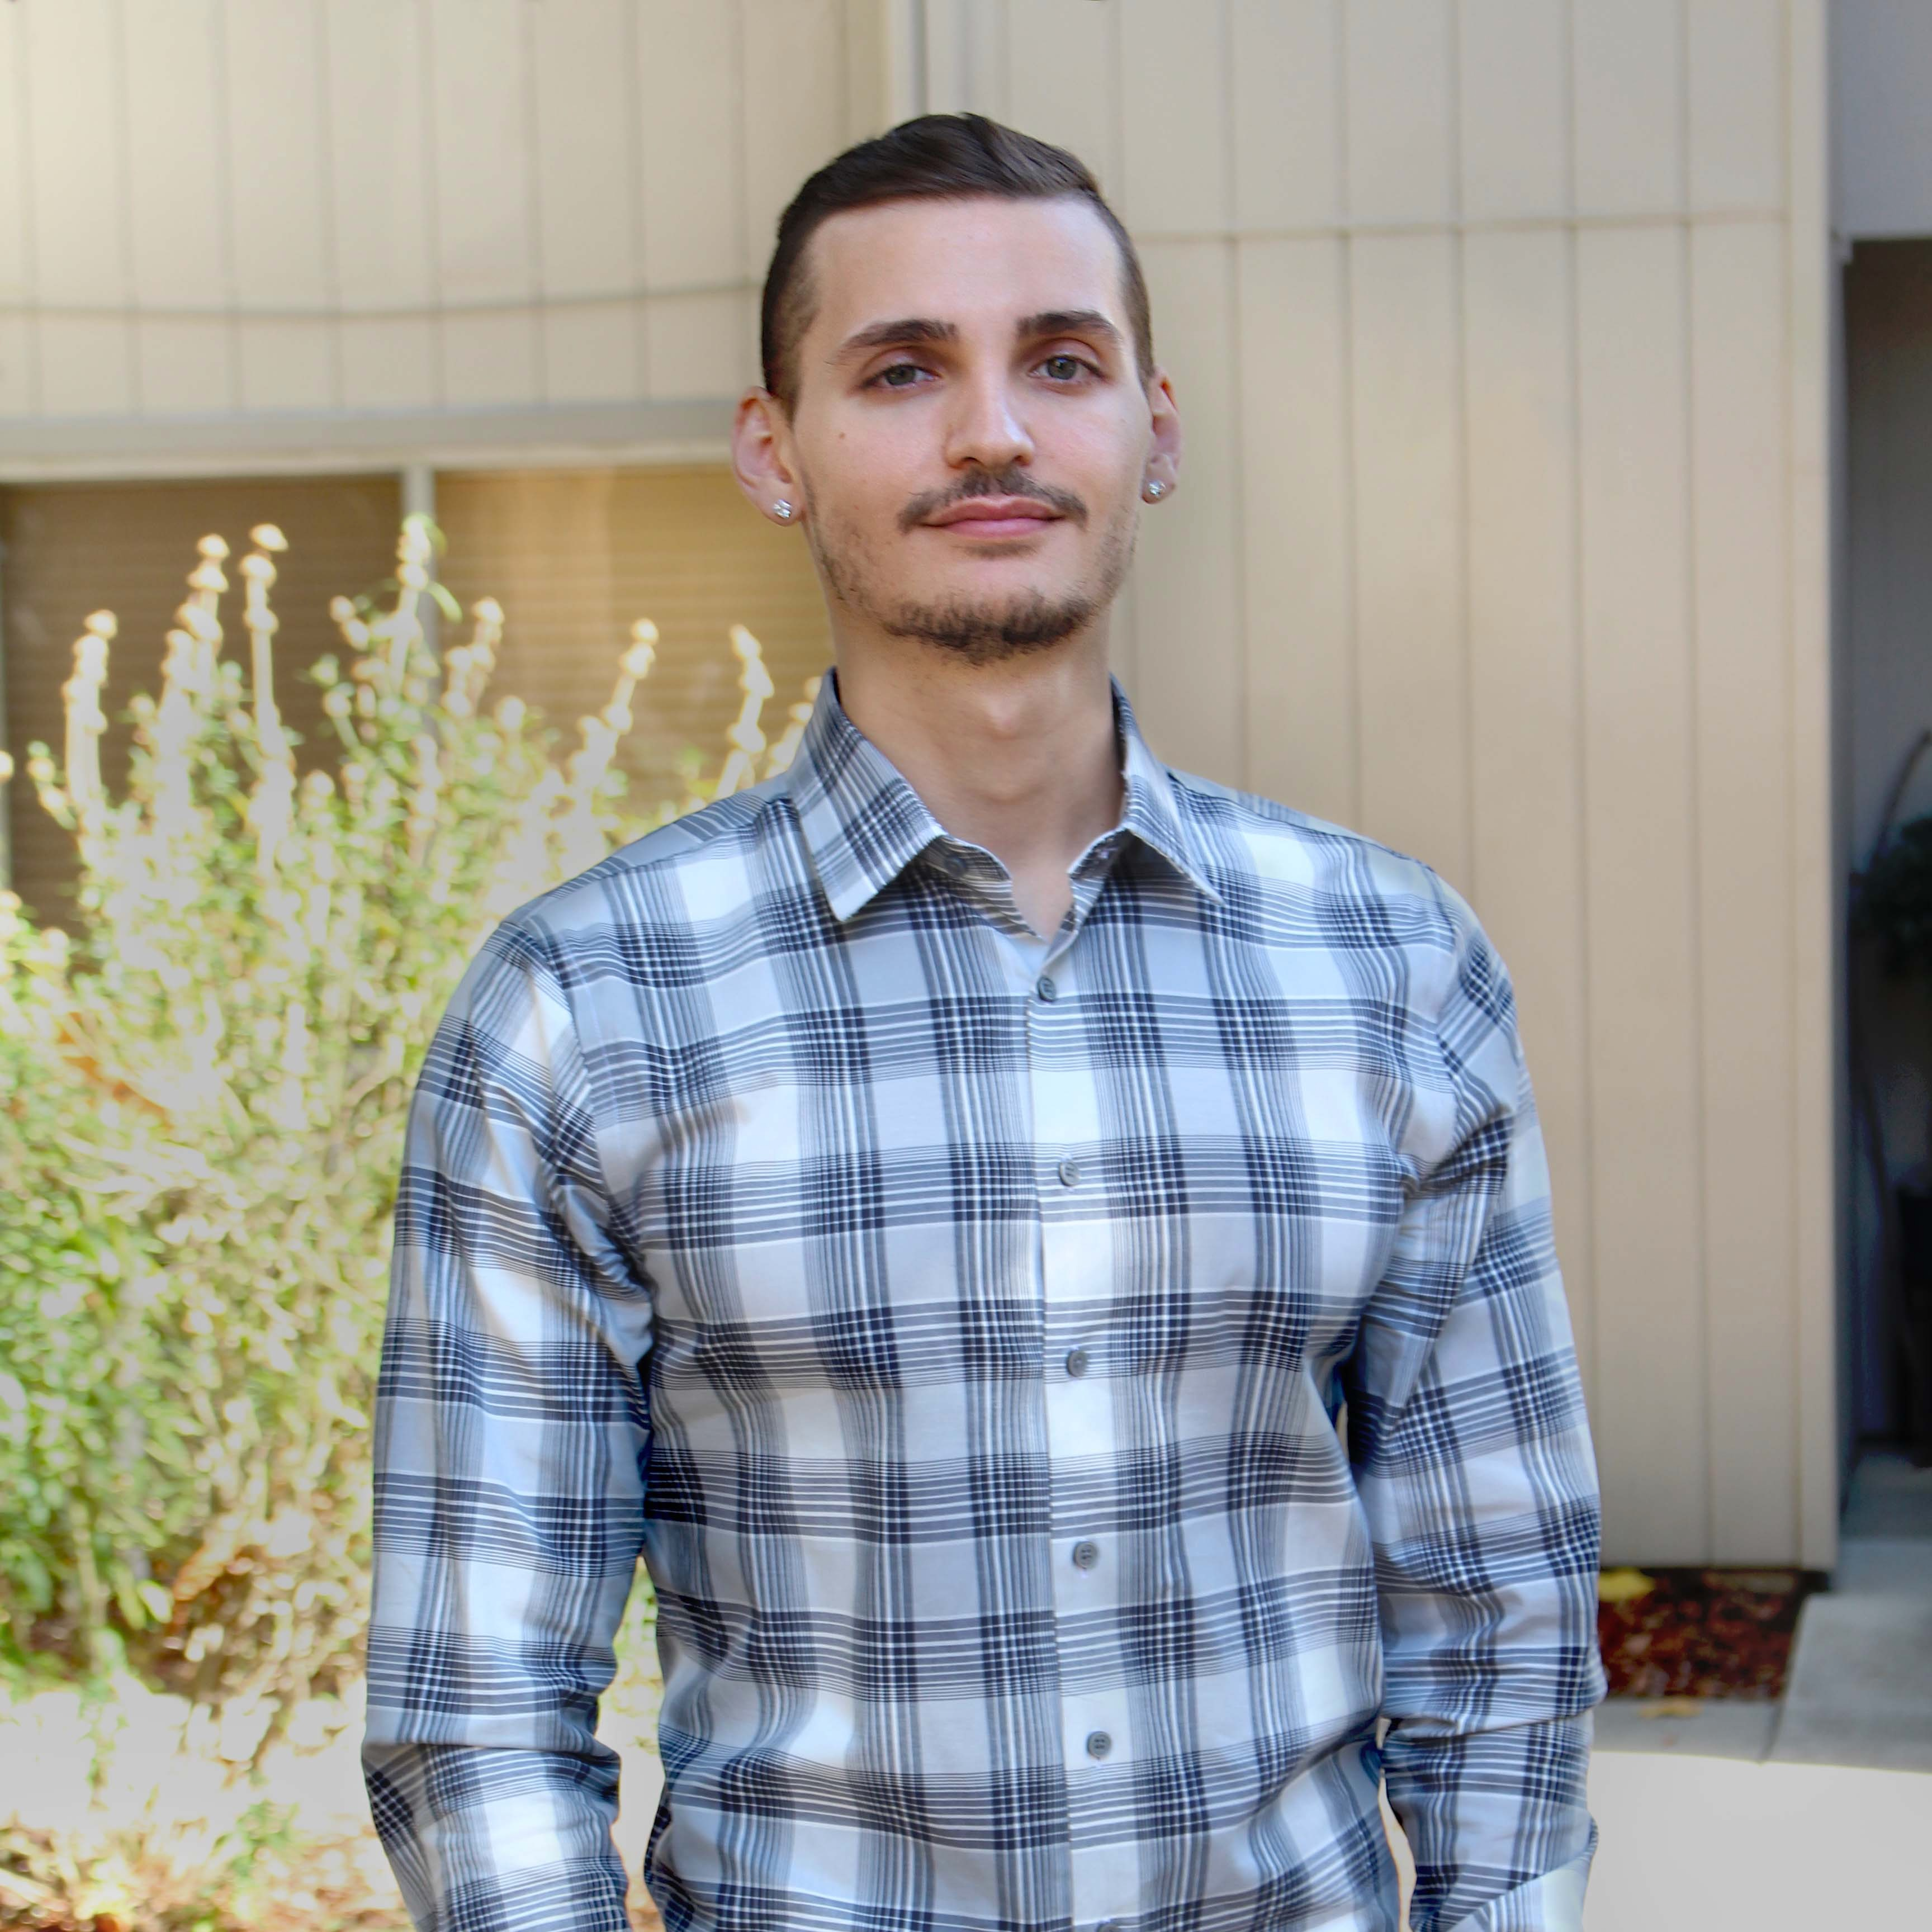
\includegraphics[width=5.1cm]{headshot.jpeg}};
        \end{tikzpicture}
\end{minipage}
\begin{minipage}[t]{0.45\textwidth} 
        {\vspace{-4.25em}\raggedleft\huge\textbf{Noam Smilovich}}
\end{minipage}
% \hfill % Horizontal space between minipages
\begin{minipage}[t]{0.35\textwidth} 
    \setlength{\baselineskip}{1.5em} % Adjust the line spacing
    \raggedright\vspace{-5em}
    \href{mailto:Noam.Smilovich@ttu.edu}{\faEnvelope\ \underline{Noam.Smilovich@ttu.edu}} \\
    \href{https://www.linkedin.com/in/noam-smilovich/}{\faLinkedin\ \underline{in/Noam-Smilovich}} \\
    \href{https://github.com/noamsmilovich}{\faGithub\ \underline{NoamSmilovich}} \\
    % \href{tel:14085020772}{\faPhone\ +1 408 502 0772} \\
    \href{https://noamsmilovich.github.io}{\faGlobe\ \underline{noamsmilovich.github.io}}
    % {\faMapMarked\ 155 Laguna St, San Francisco, CA 94102}
\end{minipage}
\section{About Me}
\justifying
I am a first-year Ph.D. student in Computer Science with a strong interdisciplinary background. My core research is dedicated to Intrinsic Robot Learning in Multimodal, Contact-Rich Environments. My research methodology leverages Information-Theoretic Control and Hybrid Dynamical Systems to enable robots to acquire complex behaviors and adapt robustly to real-world scenarios. My goal is to advance the foundations of self-motivated, perceptually-aware robotic intelligence.

%-----------EDUCATION-----------%
\section{Education}
    \resumeSubHeadingListStart

    \resumeSubheading
    {PhD in Computer Science}{2025 -- Present}
    {Texas Tech University}{Lubbock, TX}
    \resumeItemListStart
        \resumeItem{Advisor: Dr. Stas Tiomkin}
    \resumeItemListEnd

    \resumeSubheading
    {MSc in Software Engineering}{2022 -- 2024}
    {San Jos\'e State University}{San Jos\'e, CA}
    \resumeItemListStart
        \resumeItem{Thesis: Data-Driven Control of Acoustic Waves Using Movable and Flexible Scatterers.}
        \resumeItem{Thesis Advisor: Dr. Stas Tiomkin}
    \resumeItemListEnd

    \resumeSubheading
    {MSc in Electrical and Electronics Engineering}{2017 -- 2020}
    {Tel Aviv University}{Tel Aviv, Israel}
    \resumeItemListStart
        \resumeItem{Thesis: Ka-Band Power Amplifier and Digitally Controlled Attenuator in CMOS 130nm.}
        \resumeItem{Thesis Advisor: Prof. Eran Socher}
    \resumeItemListEnd

    \resumeSubheading
    {BSc in Electrical and Electronics Engineering}{2014 -- 2018}
    {Tel Aviv University}{Tel Aviv, Israel}

    \resumeSubHeadingListEnd
\section{Awards}
\resumeSubHeadingListStart 

    \resumeSubheadingTwo
        {Graduate Teaching Assistant of the Year}{2025}
        \resumeItemListStart
            \resumeItemLong{Awarded by the Department of Computer Science, Whitacre College of Engineering at Texas Tech University for outstanding performance as a Graduate Teaching Assistant.}
            % \resumeItem{Selected as the single recipient among all Computer Science graduate teaching assistants.}
        \resumeItemListEnd

    \resumeSubheadingTwo 
        {Outstanding Thesis Award}{2025}
        \resumeItemListStart 
            \resumeItemLong{University-wide award for the most outstanding master’s thesis published in 2024–2025, granted by the College of Graduate Studies at San José State University.} 
            \resumeItem{Award amount: \$1,000. Presented at the University Commencement Ceremony.} 
        \resumeItemListEnd

    \resumeSubheadingTwo 
        {Research, Scholarship, and Creative Activity (RSCA) Fellowship}{2024}
        \resumeItemListStart 
            \resumeItemLong{A competitive award for scholarly and creative activities, College of Engineering at San Jose State University. } 
            \resumeItem{Award amount: \$3,000.} 
        \resumeItemListEnd
    

\resumeSubHeadingListEnd
\newpage
\section{Publications and Presentations}

\resumeSubHeadingListStart
    \resumeSubheadingTwo {Publications}{}
        \resumeItemListStart
            \resumeItemLong{\textbf{N. Smilovich}, “Data-driven control of acoustic waves using movable and flexible scatterers,” M.Sc. thesis, San Jose State Univ., San Jose, CA, 2024.}
            \resumeItemLong{T. Shah*, \textbf{N. Smilovich}*, S. Gerges, F. Amirkulova, S. Tiomkin, "Acoustic wave manipulation through sparse robotic actuation," in {\it Proceedings of the IEEE International Conference on Robotics and Automation}, 2025.}
            \resumeItemLong{\textbf{N. Smilovich}, “Ka-band power amplifier and digitally controlled attenuator in CMOS 130nm,” M.Sc. thesis, School of Electr. Eng., Tel Aviv Univ., Tel Aviv, Israel, 2020.}
            \resumeItemLong{S. Londhe, \textbf{N. Smilovich}, S. Avner, N. Bar-Helmer, S. Jameson, and E. Socher, "34-42GHz CMOS transceiver frontend for versatile arrays," 2020 15th European Microwave Integrated Circuits Conference (EuMIC), Utrecht, Netherlands, 2021, pp. 73-76.}
        \resumeItemListEnd
% \vspace{4em}
    \resumeSubheadingTwo {Presentations}{}
        \resumeItemListStart
            \resumeItemLong{T. Shah*, \textbf{N. Smilovich}*, S. Gerges, F. Amirkulova, S. Tiomkin, “Acoustic wave manipulation through sparse robotic actuation,” poster presented at Research Showcase during Board meeting at the CS Department, Texas Tech University, Oct 2024, based on the corresponding paper.}
        \resumeItemListEnd
\resumeSubHeadingListEnd
    
%-----------EXPERIENCE-----------%
\section{Experience}
\resumeSubHeadingListStart

    \resumeSubheading
    {Graduate Teaching Assistant}{2025}
    {Department of Computer Science, Texas Tech University}{Lubbock, TX}
    \resumeItemListStart
        \resumeItemLong{Senior Capstone Course (CS 4366): Managed course logistics and project execution for 75 students, including check-in meetings between student groups and local partner company; oversaw all grading and milestone tracking.}
        \resumeItemLong{Generative AI (CS 5331/4331): Contributed directly to course content development by preparing a significant portion of lecture slides and designing a homework assignment; responsible for grading and providing detailed feedback.}
    \resumeItemListEnd

    \resumeSubheading
    {Research Assistant}{2025}
    {Computational Intelligence, Control \& Information Lab, Texas Tech University}{Lubbock, TX}
    \resumeItemListStart
        \resumeItem{Research hybrid dynamical systems in robotics, focusing on information-theoretic control and learning-based methods to analyze and optimize behavior in non-differentiable, contact-rich environments.}
    \resumeItemListEnd

    \resumeSubheading
    {Research Assistant}{2024}
    {Computational Intelligence Lab, San Jose State University}{San Jos\'e, CA}
    \resumeItemListStart
        \resumeItem{Research and development of machine learning approaches for controlling acoustic wave propagation, incorporating state-of-the-art AI architectures and predictive modeling techniques.}
    \resumeItemListEnd

    \resumeSubheading
    {Instructional Student Assistant -- Data Structures and Algorithms in C++}{2023}
    {College of Engineering, San Jose State University}{San Jos\'e, CA}
    \resumeItemListStart
        \resumeItem{Provided instructional support for the course by grading assignments, addressing student inquiries, and managing grade appeals.}
    \resumeItemListEnd

    \resumeSubheading
    {Media Architecture Systems Engineering Intern}{2023}
    {Micron Technology}{San Jos\'e, CA}
    \resumeItemListStart
        \resumeItem{Developed system architecture validation tools for NAND flash memory command sequences, improving reliability and testing efficiency.}
    \resumeItemListEnd

    \resumeSubheading
    {System Integration Engineer -- 5G Modem}{2020 -- 2021}
    {Qualcomm}{Israel}
    \resumeItemListStart
        \resumeItem{Contributed to system integration and validation efforts for 5G modem development, focusing on performance optimization and cross-functional feature implementation.}
    \resumeItemListEnd

    \resumeSubheading
    {Research Assistant}{2017 -- 2020}
    {Faculty of Engineering, Tel Aviv University}{Israel}
    \resumeItemListStart
        \resumeItem{Designed RFICs as part of a research group, with circuits sent for tape-out, followed by post-fabrication testing and characterization in the university’s high-frequency integrated circuits lab.}
    \resumeItemListEnd

    \resumeSubheading
    {Lab Instructor - Analog Circuits Lab}{2017 -- 2020}
    {Faculty of Engineering, Tel Aviv University}{Israel}
    \resumeItemListStart
        \resumeItem{Provided instructional support by conducting tutorials, grading assignments, addressing student inquiries, and managing grade appeals.}
    \resumeItemListEnd
\resumeSubHeadingListEnd
\section{Volunteer Experience}
\resumeSubHeadingListStart 

    \resumeSubheading
        {Research Mentor}{2024}
        {San Jose State University}{San Jos\'e, CA}
    \resumeItemListStart 
        \resumeItem{Conducted instructional tutorials and participated in weekly mentoring sessions to guide high school and community college students on a project at the intersection of acoustics research and machine learning.} 
    \resumeItemListEnd

\resumeSubHeadingListEnd
\section{Open-Source Contributions}
\resumeSubHeadingListStart
\resumeSubheadingTwo
    {Waves.jl}{2024}
    \resumeItemListStart 
            \resumeItem{Enhanced the Waves.jl simulator and its deep learning model by extending configuration options, improving flexibility, and supporting more diverse use cases in wave physics simulations.\\
            Repository: \href{https://github.com/gladisor/Waves.jl}{https://github.com/gladisor/Waves.jl}}
    \resumeItemListEnd
\resumeSubHeadingListEnd


% \section{Skills}
Programming Languages: Python, Julia, C, C++, C\#
Developer Tools: Git, Slurm, Conda


% \begin{multicols}{3}
% \begin{itemize}[leftmargin=0.15in, label=$\bullet$, itemsep=1pt, parsep=0pt, topsep=0pt]
% \small
%     % \item Python
%     \item Django / Flask
%     \item Java
%     \item Test-Driven Development
%     \item Unit Testing
%     \item Agile
%     % \item C
%     % \item C++
%     % \item C\#
%     % \item Julia
%     % \item PyTorch
%     % \item TensorFlow
%     % \item scikit-learn
%     % \item Pandas
%     % \item NumPy
%     % \item Flux
%     \item SQL
%     \item MongoDB
%     % \item Git
%     \item Object-Oriented Programming
%     \item Design Patterns
%     % \item Data Structures
%     % \item Agile
%     \item Linux

%     % RF STUFF:
%     \item RF
%     \item Wireless Communications
%     % \item Spectre
%     % \item Electromagnetic Simulations 
%     % \item Momentum
%     % \item Circuit Simulations
%     % \item Cadence Virtuoso
%     % \item Cadence Spectre
    
% \end{itemize}
% \end{multicols}


% \section{Languages}
% \vspace{-1.5em}
% \begin{multicols}{5}
% \begin{itemize}[leftmargin=0.15in, label=$\bullet$, itemsep=1pt, parsep=0pt, topsep=0pt]
% \small
% \centering
%     \item \textbf{Hebrew} $|$ \textit{Native}
%     \item \textbf{English} $|$ \textit{Fluent}
% \end{itemize}
% \end{multicols}

%-------------------------------------------%
\end{document}